\documentclass{beamer}

\usepackage[utf8]{inputenc}
\usepackage[spanish]{babel}
\usepackage{amsmath}
\usepackage[nosetup]{evan}
%\usetheme{Goddard}
\usetheme{Madrid}
\hypersetup{colorlinks,allcolors=.,urlcolor=magenta}
\usepackage[table]{xcolor} % Para definir colores en tablas
\usepackage{graphicx} % Para redimensionar la tabla

\title{Investigación de Operaciones II}
\subtitle{Unidad 2: Introducción a las Cadenas de Markov}
\author[Ricardo Largaespada]{Ricardo Jesús Largaespada Fernández}
\institute[UNI]{Ingeniería de Sistemas, DACTIC, UNI}
\date{22 de Abril, 2025}

\begin{document}

\frame{\titlepage}

\begin{frame}
\frametitle{Agenda}
\tableofcontents
\end{frame}

\section{Introducción}

\begin{frame}{Objetivo}
\begin{itemize}
  \item El estudiante justifica su análisis al plantear y resolver correctamente el sistema de ecuaciones de estado estable.
  \item Interpreta los resultados para proyectar costos promedio esperados.
  \item Evidencia dominio del enfoque a largo plazo en una cadena de Markov.
\end{itemize}
\end{frame}

\begin{frame}{Arremángala, Arrempújala}
    \begin{center}
        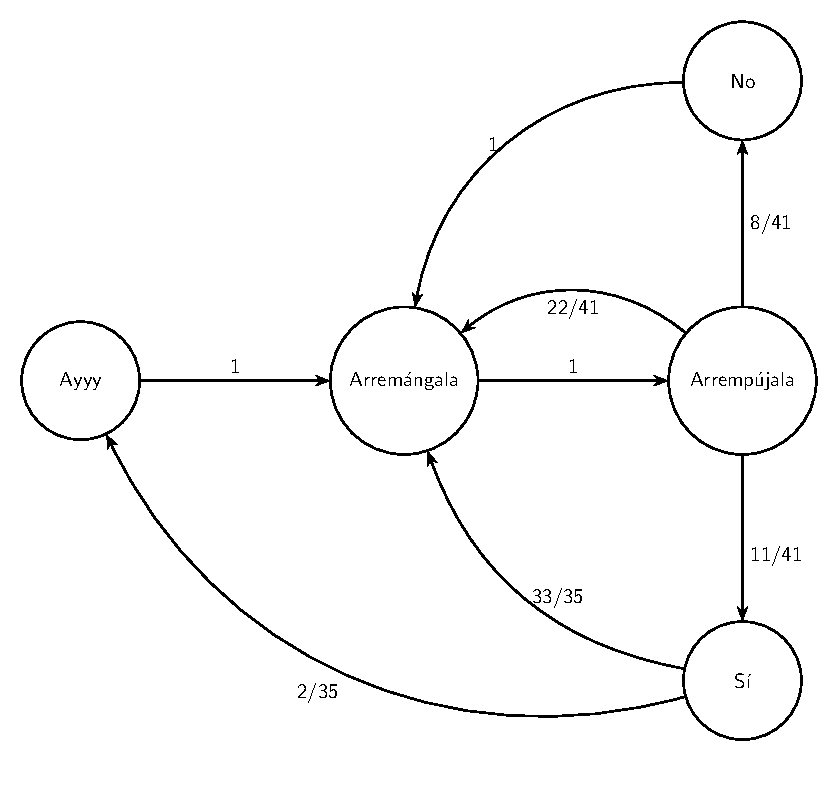
\includegraphics[scale=0.5]{images/clase13-KarkisMarkov.pdf} 
    \end{center}
\end{frame}

\section{Probabilidades de Estado Estable}

\begin{frame}{Probabilidades de Estado Estable}
\begin{itemize}
  \item Una cadena de Markov finita, irreducible y ergódica tiene una distribución límite independiente del estado inicial.
  \item Esta distribución está dada por los valores $\pi_j$ tales que:
  \[
  \pi_j = \lim_{n \to \infty} P_{ij}^{(n)}, \quad \forall i
  \]
  \item Los $\pi_j$ satisfacen el sistema de ecuaciones:
  \[
  \pi = \pi P, \quad \sum_j \pi_j = 1
  \]
\end{itemize}
\end{frame}

\begin{frame}{Interpretación}
\begin{itemize}
  \item $\pi_j$ representa la fracción de tiempo (a largo plazo) que el sistema pasa en el estado $j$.
  \item Esta probabilidad se alcanza sin importar el estado inicial.
  \item No implica que el sistema se quede fijo en un estado, sino que las visitas a cada estado se estabilizan en proporción a $\pi_j$.
\end{itemize}
\end{frame}

\begin{frame}{Cálculo}
\begin{itemize}
  \item El sistema de ecuaciones $\pi = \pi P$ con la condición $\sum \pi_j = 1$ tiene una única solución.
  \item En la práctica, se elimina una de las ecuaciones de balance y se sustituye por la ecuación de normalización.
\end{itemize}
\end{frame}

\begin{frame}{Ejemplo}
\begin{itemize}
  \item Sea $P = \begin{pmatrix} 0.8 & 0.2 \\ 0.6 & 0.4 \end{pmatrix}$
  \item Resolver:
  \[
  \pi_0 = 0.8\pi_0 + 0.6\pi_1, \quad \pi_1 = 0.2\pi_0 + 0.4\pi_1, \quad \pi_0 + \pi_1 = 1
  \]
  \item Resultado: $\pi_0 = 0.25$, $\pi_1 = 0.75$
\end{itemize}
\end{frame}

\subsection{Aplicaciones}

\begin{frame}{Ejemplo: Participación de mercado entre cervecerías}
\textbf{Contexto:}
\begin{itemize}
  \item Tres estados representan marcas de cerveza: A, B y C.
  \item A y B son cervecerías grandes, C agrupa las marcas restantes.
  \item Se modela el cambio de marca como una cadena de Markov.
\end{itemize}
\textbf{Matriz de transición}
\[
P =
\begin{pmatrix}
0.7 & 0.2 & 0.1 \\
0.2 & 0.75 & 0.05 \\
0.1 & 0.1 & 0.8
\end{pmatrix}
\]
\begin{itemize}
  \item Las filas representan el estado actual del cliente.
  \item Las columnas representan el siguiente mes.
  \item Se busca la distribución de estado estable $\pi = (\pi_A, \pi_B, \pi_C)$.
\end{itemize}
\end{frame}

\begin{frame}{Sistema de ecuaciones de estado estable}
Resolvemos el sistema:
\[
\pi = \pi P, \quad \pi_A + \pi_B + \pi_C = 1
\]
\begin{align*}
\pi_A &= 0.7\pi_A + 0.2\pi_B + 0.1\pi_C \\
\pi_B &= 0.2\pi_A + 0.75\pi_B + 0.1\pi_C \\
\pi_C &= 0.1\pi_A + 0.05\pi_B + 0.8\pi_C
\end{align*}
Eliminamos una ecuación por redundancia y usamos la de normalización.
\end{frame}

\begin{frame}{Solución e interpretación}
\begin{itemize}
  \item Resolviendo el sistema, se obtiene:
  \[
  \pi_A = \frac{9}{26} \approx 0.3461, \quad \pi_B =\frac{5}{13} \approx 0.3846, \quad \pi_C =\frac{7}{13}\approx 0.2692
  \]
  \item Interpretación:
  \begin{itemize}
    \item A tendrá aproximadamente el 34.61\% del mercado a largo plazo.
    \item B tendrá aproximadamente el 38.46\%.
    \item Las demás marcas: 26.92\%.
  \end{itemize}
  \item Este resultado permite a la empresa evaluar su posición competitiva sostenida en el tiempo.
\end{itemize}
\end{frame}

\section{Tiempo Medio de Retorno}

\begin{frame}{Tiempo Medio de Retorno}
\begin{itemize}
  \item El tiempo medio de retorno a un estado $j$ es el número esperado de pasos hasta regresar a $j$.
  \item Se calcula como:
  \[
  \mu_{jj} = \frac{1}{\pi_j}
  \]
  \item A mayor $\pi_j$, menor es el tiempo esperado de retorno.
\end{itemize}
\end{frame}

\begin{frame}{Ejemplo}
\begin{itemize}
  \item Con $\pi_0 = 0.25$, $\pi_1 = 0.75$:
  \[
  \mu_{00} = \frac{1}{0.25} = 4, \quad \mu_{11} = \frac{1}{0.75} \approx 1.33
  \]
  \item El estado 1 se visita más frecuentemente que el estado 0.
\end{itemize}
\end{frame}

\section{Costo Promedio Esperado}

\begin{frame}{Costo Promedio Esperado}
\begin{itemize}
  \item Sea $C(j)$ el costo incurrido cuando el sistema está en el estado $j$.
  \item A largo plazo, el costo promedio por unidad de tiempo está dado por:
  \[
  \sum_j \pi_j C(j)
  \]
  \item Este resultado es válido bajo la existencia de la distribución de estado estable.
\end{itemize}
\end{frame}

\begin{frame}{Ejemplo}
\begin{itemize}
  \item Supón: $C(0)=0$, $C(1)=2$, $C(2)=8$, $C(3)=18$
  \item Y $\pi_0 = 0.286$, $\pi_1 = 0.285$, $\pi_2 = 0.263$, $\pi_3 = 0.166$
  \item Costo esperado:
  \[
  0.286(0) + 0.285(2) + 0.263(8) + 0.166(18) = 5.662
  \]
\end{itemize}
\end{frame}

\begin{frame}{Ejemplo: Ingresos esperados en función del clima}
\textbf{Contexto:}
\begin{itemize}
  \item MiniGolf genera ingresos según el clima: 
  \begin{itemize}
    \item Soleado: \$2000
    \item Nublado: \$1600
    \item Lluvioso: \$400
  \end{itemize}
  \item Transiciones diarias del clima:
  \[
  P = \begin{pmatrix}
  0.8 & 0.2 & 0.0 \\
  0.3 & 0.0 & 0.7 \\
  0.1 & 0.1 & 0.8
  \end{pmatrix}
  \]
  \item Estados: 0 = Soleado, 1 = Nublado, 2 = Lluvioso
\end{itemize}
\end{frame}

\begin{frame}{Solución e interpretación}
\textbf{Estado estable:}
\[
\pi = (\pi_0, \pi_1, \pi_2) \Rightarrow \pi_0 \approx 0.419, \quad \pi_1 \approx 0.129, \quad \pi_2 \approx 0.451
\]

\textbf{(a) Ingreso diario esperado:}
\[
E(I) = 2000(0.419) + 1600(0.129) + 400(0.451) = 838 + 206.4 + 180.4 \approx \boxed{\$1225}
\]

\textbf{(b) Promedio de días no soleados:}
\[
1 - \pi_0 = 1 - 0.419 = \boxed{0.581} \text{ o 58.1\% del tiempo}
\]
\end{frame}

% PROBLEMA 2
\begin{frame}{Ejemplo: Hábitos alimenticios de Joe}
\textbf{Contexto:}
\begin{itemize}
  \item Joe come en 4 tipos de restaurantes: mexicana, italiana, china, tailandesa.
  \item Costos promedio: 
  \begin{itemize}
    \item Mexicana: \$10
    \item Italiana: \$15
    \item China: \$9
    \item Tailandesa: \$11
  \end{itemize}
  \item 70\% de probabilidad de repetir tipo de comida, 10\% para cada una de las otras.
\end{itemize}
\end{frame}

\begin{frame}{Formulación como cadena de Markov}
\[
P = 
\begin{pmatrix}
0.7 & 0.1 & 0.1 & 0.1 \\
0.1 & 0.7 & 0.1 & 0.1 \\
0.1 & 0.1 & 0.7 & 0.1 \\
0.1 & 0.1 & 0.1 & 0.7
\end{pmatrix}
\]
\begin{itemize}
  \item Matriz simétrica, todos los estados tienen la misma estructura.
  \item Estado estable:
  \[
  \pi = (0.25, 0.25, 0.25, 0.25)
  \]
\end{itemize}
\end{frame}

\begin{frame}{Cálculo de expectativas}
\textbf{(a) Gasto promedio diario:}
\[
E(C) = 0.25(10 + 15 + 9 + 11) = \boxed{\$11.25}
\]

\textbf{(b) Frecuencia con que consume comida mexicana:}
\[
\pi_1 = \boxed{25\%}
\]
\textbf{Interpretación:} Aunque hay alta probabilidad de repetir, el equilibrio entre todas las opciones estabiliza la elección.
\end{frame}

\begin{frame}{Ejemplo: Dinámica poblacional en Mobile}
\textbf{Contexto:}
\begin{itemize}
  \item La población se clasifica en tres grupos:
  \begin{itemize}
    \item Rural (R)
    \item Suburbana (S)
    \item Citadina (C)
  \end{itemize}
  \item Cada 10 años, las personas pueden cambiar de zona.
  \item El movimiento se modela con una cadena de Markov.
\end{itemize}
\end{frame}

\begin{frame}{Modelado de la cadena de Markov}
\textbf{Matriz de transición:}
\[
P =
\begin{pmatrix}
0.85 & 0.10 & 0.05 \\
0.30 & 0.55 & 0.15 \\
0.20 & 0.00 & 0.80
\end{pmatrix}
\]
\begin{itemize}
  \item Las filas representan el origen: R, S, C.
  \item Las columnas el destino.
  \item Cada fila suma 1.
\end{itemize}
\end{frame}

\begin{frame}{Proyección de la población}
\textbf{Condiciones iniciales:}
\[
x_0 = \begin{pmatrix} 20000 & 100000 & 30000 \end{pmatrix}
\]

\textbf{Población después de 10 años:}
\[
x_{10} = x_0 \cdot P = \boxed{\begin{pmatrix} 48900 & 64900 & 37000 \end{pmatrix}}
\]

\textbf{Después de 20 años:}
\[
x_{20} = x_{10} \cdot P = \boxed{\begin{pmatrix} 58966 & 55402 & 40632 \end{pmatrix}}
\]

\textbf{Interpretación:} Aumenta la población rural, disminuye la suburbana.
\end{frame}

\begin{frame}{Estado estable de la población}
\textbf{Resolviendo:} $\pi = \pi P, \quad \pi_R + \pi_S + \pi_C = 1$
\[
\pi \approx \begin{pmatrix} 0.655 & 0.202 & 0.143 \end{pmatrix}
\]

\textbf{Interpretación:}
\begin{itemize}
  \item A largo plazo, el 65.5\% de la población vivirá en zonas rurales.
  \item Solo el 14.3\% permanecerá en zonas citadinas.
  \item Refleja un patrón migratorio hacia áreas más tranquilas o rurales.
\end{itemize}
\end{frame}

\section{Costo con Funciones de Varias Variables}

\begin{frame}{Funciones de Costo Complejas}
\begin{itemize}
  \item En algunos casos, el costo no solo depende del estado actual, sino también de otras variables como demanda $D_t$.
  \item Entonces, el costo se modela como $C(X_t, D_t)$
  \item A largo plazo:
  \[
  \sum_j \pi_j \mathbb{E}[C(j, D)]
  \]
\end{itemize}
\end{frame}

\begin{frame}{Ejemplo}
\begin{itemize}
  \item Supón que $C(X_t, D_t)$ depende de si se hace un pedido y la demanda:
  \[
  C(0, D_t) = 85 + 50 \max(D_t - 3, 0)
  \]
  \[
  C(x, D_t) = 50 \max(D_t - x, 0) \text{ si } x \geq 1
  \]
  \item Si se usa distribución de Poisson para $D_t$:
  \[
  k(0) = 86.2, \quad k(1) = 18.4, \quad k(2) = 5.2, \quad k(3) = 1.2
  \]
  \[
  \text{Costo promedio} = \sum_j \pi_j k(j) = 31.46
  \]
\end{itemize}
\end{frame}


\section{Conclusión}

\begin{frame}{Conclusión}
\begin{itemize}
  \item Las probabilidades de estado estable permiten describir el comportamiento a largo plazo del sistema.
  \item El costo promedio esperado se puede calcular con base en esas probabilidades.
  \item Las funciones de costo pueden ser simples o depender de múltiples variables aleatorias.
\end{itemize}
\end{frame}

\begin{frame}
\centering
\Huge ¡Gracias!
\end{frame}

\end{document}
